% Options for packages loaded elsewhere
% Options for packages loaded elsewhere
\PassOptionsToPackage{unicode}{hyperref}
\PassOptionsToPackage{hyphens}{url}
%
\documentclass[
  ignorenonframetext,
  aspectratio=169,
  russian,
]{beamer}
\newif\ifbibliography
\usepackage{pgfpages}
\setbeamertemplate{caption}[numbered]
\setbeamertemplate{caption label separator}{: }
\setbeamercolor{caption name}{fg=normal text.fg}
\beamertemplatenavigationsymbolshorizontal
% Prevent slide breaks in the middle of a paragraph
\widowpenalties 1 10000
\raggedbottom
\AtBeginPart{
  \frame{\partpage}
}
\AtBeginSection{
  \ifbibliography
  \else
    \frame{\sectionpage}
  \fi
}
\AtBeginSubsection{
  \frame{\subsectionpage}
}
\usepackage{iftex}
\ifPDFTeX
  \usepackage[T1]{fontenc}
  \usepackage[utf8]{inputenc}
  \usepackage{textcomp} % provide euro and other symbols
\else % if luatex or xetex
  \usepackage{unicode-math} % this also loads fontspec
  \defaultfontfeatures{Scale=MatchLowercase}
  \defaultfontfeatures[\rmfamily]{Ligatures=TeX,Scale=1}
\fi
\usepackage{lmodern}

\usetheme[]{Montpellier}
\usecolortheme[]{seagull}
\ifPDFTeX\else
  % xetex/luatex font selection
\fi
% Use upquote if available, for straight quotes in verbatim environments
\IfFileExists{upquote.sty}{\usepackage{upquote}}{}
\IfFileExists{microtype.sty}{% use microtype if available
  \usepackage[]{microtype}
  \UseMicrotypeSet[protrusion]{basicmath} % disable protrusion for tt fonts
}{}

\usepackage{color}
\usepackage{fancyvrb}
\newcommand{\VerbBar}{|}
\newcommand{\VERB}{\Verb[commandchars=\\\{\}]}
\DefineVerbatimEnvironment{Highlighting}{Verbatim}{commandchars=\\\{\}}
% Add ',fontsize=\small' for more characters per line
\usepackage{framed}
\definecolor{shadecolor}{RGB}{241,243,245}
\newenvironment{Shaded}{\begin{snugshade}}{\end{snugshade}}
\newcommand{\AlertTok}[1]{\textcolor[rgb]{0.68,0.00,0.00}{#1}}
\newcommand{\AnnotationTok}[1]{\textcolor[rgb]{0.37,0.37,0.37}{#1}}
\newcommand{\AttributeTok}[1]{\textcolor[rgb]{0.40,0.45,0.13}{#1}}
\newcommand{\BaseNTok}[1]{\textcolor[rgb]{0.68,0.00,0.00}{#1}}
\newcommand{\BuiltInTok}[1]{\textcolor[rgb]{0.00,0.23,0.31}{#1}}
\newcommand{\CharTok}[1]{\textcolor[rgb]{0.13,0.47,0.30}{#1}}
\newcommand{\CommentTok}[1]{\textcolor[rgb]{0.37,0.37,0.37}{#1}}
\newcommand{\CommentVarTok}[1]{\textcolor[rgb]{0.37,0.37,0.37}{\textit{#1}}}
\newcommand{\ConstantTok}[1]{\textcolor[rgb]{0.56,0.35,0.01}{#1}}
\newcommand{\ControlFlowTok}[1]{\textcolor[rgb]{0.00,0.23,0.31}{\textbf{#1}}}
\newcommand{\DataTypeTok}[1]{\textcolor[rgb]{0.68,0.00,0.00}{#1}}
\newcommand{\DecValTok}[1]{\textcolor[rgb]{0.68,0.00,0.00}{#1}}
\newcommand{\DocumentationTok}[1]{\textcolor[rgb]{0.37,0.37,0.37}{\textit{#1}}}
\newcommand{\ErrorTok}[1]{\textcolor[rgb]{0.68,0.00,0.00}{#1}}
\newcommand{\ExtensionTok}[1]{\textcolor[rgb]{0.00,0.23,0.31}{#1}}
\newcommand{\FloatTok}[1]{\textcolor[rgb]{0.68,0.00,0.00}{#1}}
\newcommand{\FunctionTok}[1]{\textcolor[rgb]{0.28,0.35,0.67}{#1}}
\newcommand{\ImportTok}[1]{\textcolor[rgb]{0.00,0.46,0.62}{#1}}
\newcommand{\InformationTok}[1]{\textcolor[rgb]{0.37,0.37,0.37}{#1}}
\newcommand{\KeywordTok}[1]{\textcolor[rgb]{0.00,0.23,0.31}{\textbf{#1}}}
\newcommand{\NormalTok}[1]{\textcolor[rgb]{0.00,0.23,0.31}{#1}}
\newcommand{\OperatorTok}[1]{\textcolor[rgb]{0.37,0.37,0.37}{#1}}
\newcommand{\OtherTok}[1]{\textcolor[rgb]{0.00,0.23,0.31}{#1}}
\newcommand{\PreprocessorTok}[1]{\textcolor[rgb]{0.68,0.00,0.00}{#1}}
\newcommand{\RegionMarkerTok}[1]{\textcolor[rgb]{0.00,0.23,0.31}{#1}}
\newcommand{\SpecialCharTok}[1]{\textcolor[rgb]{0.37,0.37,0.37}{#1}}
\newcommand{\SpecialStringTok}[1]{\textcolor[rgb]{0.13,0.47,0.30}{#1}}
\newcommand{\StringTok}[1]{\textcolor[rgb]{0.13,0.47,0.30}{#1}}
\newcommand{\VariableTok}[1]{\textcolor[rgb]{0.07,0.07,0.07}{#1}}
\newcommand{\VerbatimStringTok}[1]{\textcolor[rgb]{0.13,0.47,0.30}{#1}}
\newcommand{\WarningTok}[1]{\textcolor[rgb]{0.37,0.37,0.37}{\textit{#1}}}

\usepackage{longtable,booktabs,array}
\usepackage{calc} % for calculating minipage widths
\usepackage{caption}
% Make caption package work with longtable
\makeatletter
\def\fnum@table{\tablename~\thetable}
\makeatother
\usepackage{graphicx}
\makeatletter
\newsavebox\pandoc@box
\newcommand*\pandocbounded[1]{% scales image to fit in text height/width
  \sbox\pandoc@box{#1}%
  \Gscale@div\@tempa{\textheight}{\dimexpr\ht\pandoc@box+\dp\pandoc@box\relax}%
  \Gscale@div\@tempb{\linewidth}{\wd\pandoc@box}%
  \ifdim\@tempb\p@<\@tempa\p@\let\@tempa\@tempb\fi% select the smaller of both
  \ifdim\@tempa\p@<\p@\scalebox{\@tempa}{\usebox\pandoc@box}%
  \else\usebox{\pandoc@box}%
  \fi%
}
% Set default figure placement to htbp
\def\fps@figure{htbp}
\makeatother



\ifLuaTeX
\usepackage[bidi=basic,provide=*]{babel}
\else
\usepackage[bidi=default,provide=*]{babel}
\fi
% get rid of language-specific shorthands (see #6817):
\let\LanguageShortHands\languageshorthands
\def\languageshorthands#1{}


\setlength{\emergencystretch}{3em} % prevent overfull lines

\providecommand{\tightlist}{%
  \setlength{\itemsep}{0pt}\setlength{\parskip}{0pt}}



 

\usepackage[]{csquotes}

\usepackage{libertine}
\makeatletter
\@ifpackageloaded{caption}{}{\usepackage{caption}}
\AtBeginDocument{%
\ifdefined\contentsname
  \renewcommand*\contentsname{Содержание}
\else
  \newcommand\contentsname{Содержание}
\fi
\ifdefined\listfigurename
  \renewcommand*\listfigurename{Список иллюстраций}
\else
  \newcommand\listfigurename{Список иллюстраций}
\fi
\ifdefined\listtablename
  \renewcommand*\listtablename{Список таблиц}
\else
  \newcommand\listtablename{Список таблиц}
\fi
\ifdefined\figurename
  \renewcommand*\figurename{Рисунок}
\else
  \newcommand\figurename{Рисунок}
\fi
\ifdefined\tablename
  \renewcommand*\tablename{Таблица}
\else
  \newcommand\tablename{Таблица}
\fi
}
\@ifpackageloaded{float}{}{\usepackage{float}}
\floatstyle{ruled}
\@ifundefined{c@chapter}{\newfloat{codelisting}{h}{lop}}{\newfloat{codelisting}{h}{lop}[chapter]}
\floatname{codelisting}{Список}
\newcommand*\listoflistings{\listof{codelisting}{Листинги}}
\makeatother
\makeatletter
\makeatother
\makeatletter
\@ifpackageloaded{caption}{}{\usepackage{caption}}
\@ifpackageloaded{subcaption}{}{\usepackage{subcaption}}
\makeatother

\usepackage{bookmark}
\IfFileExists{xurl.sty}{\usepackage{xurl}}{} % add URL line breaks if available
\urlstyle{same}
\hypersetup{
  pdftitle={Лабораторная работа №12},
  pdfauthor={Mohamed Musa},
  pdflang={ru-RU},
  hidelinks,
  pdfcreator={LaTeX via pandoc}}


\title{Лабораторная работа №12}
\subtitle{Выполнение и отладка программ}
\author{Mohamed Musa}
\date{}

\begin{document}
\frame{\titlepage}

\renewcommand*\contentsname{Содержание}
\begin{frame}[allowframebreaks]
  \frametitle{Содержание}
  \setcounter{tocdepth}{2}
  \tableofcontents
\end{frame}
\setcounter{tocdepth}{2}
\tableofcontents
}

\section{1. Информация}\label{ux438ux43dux444ux43eux440ux43cux430ux446ux438ux44f}

\begin{frame}{1.1 Докладчик}
\phantomsection\label{ux434ux43eux43aux43bux430ux434ux447ux438ux43a}
\begin{columns}[c]
\begin{column}{1\linewidth}
\begin{itemize}[<+->]
\tightlist
\item
  Mohamed Musa
\item
  Студент группы НКАбд-05-24
\item
  Номер студенческого билета: 1032248286
\item
  Российский университет дружбы народов
\item
  \href{mailto:1032248286@pfur.ru}{\nolinkurl{1032248286@pfur.ru}}
\end{itemize}
\end{column}
\end{columns}
\end{frame}

\section{2. Вводная
часть}\label{ux432ux432ux43eux434ux43dux430ux44f-ux447ux430ux441ux442ux44c}

\begin{frame}{2.1 Актуальность}
\phantomsection\label{ux430ux43aux442ux443ux430ux43bux44cux43dux43eux441ux442ux44c}
\begin{itemize}[<+->]
\tightlist
\item
  Выполнение программ --- основа работы в операционной системе Linux
\item
  Отладка --- критически важный навык для разработчиков и системных
  администраторов
\item
  Управление процессами необходимо для эффективной работы с системой
\item
  Мониторинг процессов позволяет оптимизировать производительность
\end{itemize}
\end{frame}

\begin{frame}{2.2 Объект и предмет исследования}
\phantomsection\label{ux43eux431ux44aux435ux43aux442-ux438-ux43fux440ux435ux434ux43cux435ux442-ux438ux441ux441ux43bux435ux434ux43eux432ux430ux43dux438ux44f}
\begin{itemize}[<+->]
\tightlist
\item
  \textbf{Объект исследования}: процессы и программы в операционной
  системе Linux
\item
  \textbf{Предмет исследования}: методы выполнения, отладки и
  мониторинга программ
\end{itemize}
\end{frame}

\begin{frame}{2.3 Цели и задачи}
\phantomsection\label{ux446ux435ux43bux438-ux438-ux437ux430ux434ux430ux447ux438}
\textbf{Цель работы}: освоить методы выполнения и отладки программ в
Linux

\textbf{Задачи:}

\begin{itemize}[<+->]
\tightlist
\item
  Освоить запуск программ и скриптов в различных режимах
\item
  Изучить отслеживание и мониторинг выполнения процессов
\item
  Практиковать инструменты отладки программ
\item
  Освоить управление фоновыми задачами
\item
  Изучить перенаправление ввода-вывода и конвейеры
\end{itemize}
\end{frame}

\begin{frame}{2.4 Материалы и методы}
\phantomsection\label{ux43cux430ux442ux435ux440ux438ux430ux43bux44b-ux438-ux43cux435ux442ux43eux434ux44b}
\textbf{Материалы:}

\begin{itemize}[<+->]
\tightlist
\item
  Операционная система Linux
\item
  Bash скрипты для тестирования
\item
  Программы на языке C
\item
  Компилятор GCC
\end{itemize}

\textbf{Методы:}

\begin{itemize}[<+->]
\tightlist
\item
  Практическое выполнение команд
\item
  Отладка с помощью GDB
\item
  Трассировка системных вызовов
\item
  Мониторинг процессов
\end{itemize}
\end{frame}

\section{3. Теоретические
сведения}\label{ux442ux435ux43eux440ux435ux442ux438ux447ux435ux441ux43aux438ux435-ux441ux432ux435ux434ux435ux43dux438ux44f}

\begin{frame}{3.1 Процессы в Linux}
\phantomsection\label{ux43fux440ux43eux446ux435ux441ux441ux44b-ux432-linux}
\textbf{Процесс} --- это запущенный экземпляр программы, выполняющийся в
операционной системе

\textbf{Основные характеристики:}

\begin{itemize}[<+->]
\tightlist
\item
  \textbf{PID (Process ID)} --- уникальный идентификатор процесса
\item
  \textbf{PPID (Parent Process ID)} --- идентификатор родительского
  процесса
\item
  \textbf{UID (User ID)} --- идентификатор пользователя
\item
  \textbf{Состояние} --- running, sleeping, stopped, zombie
\item
  \textbf{Приоритет} --- значение nice от -20 (высший) до 19 (низший)
\end{itemize}
\end{frame}

\begin{frame}{3.2 Типы процессов}
\phantomsection\label{ux442ux438ux43fux44b-ux43fux440ux43eux446ux435ux441ux441ux43eux432}
\begin{itemize}[<+->]
\tightlist
\item
  \textbf{Интерактивные} --- запущенные из терминала, требуют
  взаимодействия
\item
  \textbf{Фоновые (background)} --- выполняются в фоне, не блокируют
  терминал
\item
  \textbf{Демоны (daemons)} --- системные процессы, работающие постоянно
\end{itemize}
\end{frame}

\begin{frame}[fragile]{3.3 Запуск программ}
\phantomsection\label{ux437ux430ux43fux443ux441ux43a-ux43fux440ux43eux433ux440ux430ux43cux43c}
\textbf{Обычный запуск:}

\begin{Shaded}
\begin{Highlighting}[]
\ExtensionTok{./program}          \CommentTok{\# запуск исполняемого файла}
\FunctionTok{bash}\NormalTok{ script.sh     }\CommentTok{\# запуск bash скрипта}
\end{Highlighting}
\end{Shaded}

\textbf{Фоновое выполнение:}

\begin{Shaded}
\begin{Highlighting}[]
\ExtensionTok{./program} \KeywordTok{\&}        \CommentTok{\# запуск в фоне}
\end{Highlighting}
\end{Shaded}

\textbf{С nohup:}

\begin{Shaded}
\begin{Highlighting}[]
\FunctionTok{nohup}\NormalTok{ ./program }\KeywordTok{\&}  \CommentTok{\# продолжит работу после закрытия терминала}
\end{Highlighting}
\end{Shaded}
\end{frame}

\begin{frame}[fragile]{3.4 Управление задачами}
\phantomsection\label{ux443ux43fux440ux430ux432ux43bux435ux43dux438ux435-ux437ux430ux434ux430ux447ux430ux43cux438}
\textbf{Основные команды:}

\begin{itemize}[<+->]
\tightlist
\item
  \texttt{jobs} --- просмотр фоновых задач
\item
  \texttt{jobs\ -l} --- с отображением PID
\item
  \texttt{fg\ \%1} --- перевод задачи на передний план
\item
  \texttt{bg\ \%1} --- продолжить выполнение в фоне
\item
  \texttt{Ctrl+Z} --- приостановить текущую задачу
\item
  \texttt{Ctrl+C} --- прервать текущую задачу
\end{itemize}
\end{frame}

\begin{frame}{3.5 Перенаправление вывода}
\phantomsection\label{ux43fux435ux440ux435ux43dux430ux43fux440ux430ux432ux43bux435ux43dux438ux435-ux432ux44bux432ux43eux434ux430}
\textbf{Стандартные потоки:}

\begin{itemize}[<+->]
\tightlist
\item
  \textbf{stdin (0)} --- стандартный ввод (клавиатура)
\item
  \textbf{stdout (1)} --- стандартный вывод (экран)
\item
  \textbf{stderr (2)} --- стандартный вывод ошибок (экран)
\end{itemize}
\end{frame}

\begin{frame}[fragile]{3.6 Операторы перенаправления}
\phantomsection\label{ux43eux43fux435ux440ux430ux442ux43eux440ux44b-ux43fux435ux440ux435ux43dux430ux43fux440ux430ux432ux43bux435ux43dux438ux44f}
\begin{itemize}[<+->]
\tightlist
\item
  \texttt{\textgreater{}} --- перенаправление вывода (перезапись)
\item
  \texttt{\textgreater{}\textgreater{}} --- добавление в конец файла
\item
  \texttt{\textless{}} --- перенаправление ввода
\item
  \texttt{2\textgreater{}} --- перенаправление ошибок
\item
  \texttt{2\textgreater{}\&1} --- объединение stdout и stderr
\item
  \texttt{\textbar{}} --- конвейер (pipe)
\end{itemize}
\end{frame}

\begin{frame}[fragile]{3.7 Примеры перенаправления}
\phantomsection\label{ux43fux440ux438ux43cux435ux440ux44b-ux43fux435ux440ux435ux43dux430ux43fux440ux430ux432ux43bux435ux43dux438ux44f}
\begin{Shaded}
\begin{Highlighting}[]
\CommentTok{\# Перенаправление вывода}
\ExtensionTok{./program} \OperatorTok{\textgreater{}}\NormalTok{ output.txt}

\CommentTok{\# Перенаправление ошибок}
\ExtensionTok{./program} \DecValTok{2}\OperatorTok{\textgreater{}}\NormalTok{ errors.txt}

\CommentTok{\# Оба потока в один файл}
\ExtensionTok{./program} \OperatorTok{\textgreater{}}\NormalTok{ output.txt }\DecValTok{2}\OperatorTok{\textgreater{}\&}\DecValTok{1}

\CommentTok{\# Отбросить вывод}
\ExtensionTok{./program} \OperatorTok{\textgreater{}}\NormalTok{ /dev/null }\DecValTok{2}\OperatorTok{\textgreater{}\&}\DecValTok{1}
\end{Highlighting}
\end{Shaded}
\end{frame}

\begin{frame}[fragile]{3.8 Конвейеры (Pipes)}
\phantomsection\label{ux43aux43eux43dux432ux435ux439ux435ux440ux44b-pipes}
\textbf{Конвейер} --- передача вывода одной команды на вход другой:

\begin{Shaded}
\begin{Highlighting}[]
\ExtensionTok{command1} \KeywordTok{|} \ExtensionTok{command2}
\end{Highlighting}
\end{Shaded}

\textbf{Примеры:}

\begin{itemize}[<+->]
\tightlist
\item
  \texttt{ps\ aux\ \textbar{}\ grep\ firefox} --- поиск процесса
\item
  \texttt{ps\ aux\ \textbar{}\ wc\ -l} --- подсчет процессов
\item
  \texttt{cat\ file.txt\ \textbar{}\ sort\ \textbar{}\ uniq} ---
  сортировка и удаление дубликатов
\end{itemize}
\end{frame}

\begin{frame}[fragile]{3.9 Мониторинг процессов: ps}
\phantomsection\label{ux43cux43eux43dux438ux442ux43eux440ux438ux43dux433-ux43fux440ux43eux446ux435ux441ux441ux43eux432-ps}
\textbf{Команда ps} --- информация о процессах:

\begin{itemize}[<+->]
\tightlist
\item
  \texttt{ps} --- процессы текущего терминала
\item
  \texttt{ps\ -e} --- все процессы
\item
  \texttt{ps\ aux} --- подробная информация
\item
  \texttt{ps\ -u\ username} --- процессы пользователя
\item
  \texttt{ps\ -p\ PID} --- информация о конкретном процессе
\end{itemize}
\end{frame}

\begin{frame}[fragile]{3.10 Мониторинг процессов: top}
\phantomsection\label{ux43cux43eux43dux438ux442ux43eux440ux438ux43dux433-ux43fux440ux43eux446ux435ux441ux441ux43eux432-top}
\textbf{Команда top} --- интерактивный мониторинг в реальном времени

\textbf{Клавиши управления:}

\begin{itemize}[<+->]
\tightlist
\item
  \texttt{q} --- выход
\item
  \texttt{k} --- убить процесс
\item
  \texttt{M} --- сортировка по памяти
\item
  \texttt{P} --- сортировка по CPU
\item
  \texttt{u} --- фильтр по пользователю
\end{itemize}
\end{frame}

\begin{frame}{3.11 Мониторинг процессов: htop}
\phantomsection\label{ux43cux43eux43dux438ux442ux43eux440ux438ux43dux433-ux43fux440ux43eux446ux435ux441ux441ux43eux432-htop}
\textbf{Команда htop} --- улучшенная версия top

\textbf{Преимущества:}

\begin{itemize}[<+->]
\tightlist
\item
  Цветной интерфейс
\item
  Использование мыши
\item
  Древовидное отображение процессов
\item
  Легкое управление процессами
\end{itemize}
\end{frame}

\begin{frame}[fragile]{3.12 Поиск процессов}
\phantomsection\label{ux43fux43eux438ux441ux43a-ux43fux440ux43eux446ux435ux441ux441ux43eux432}
\begin{itemize}[<+->]
\tightlist
\item
  \texttt{pgrep\ firefox} --- найти PID процессов firefox
\item
  \texttt{pidof\ firefox} --- найти PID по имени программы
\item
  \texttt{ps\ aux\ \textbar{}\ grep\ firefox} --- поиск с помощью grep
\end{itemize}
\end{frame}

\begin{frame}[fragile]{3.13 Управление процессами: kill}
\phantomsection\label{ux443ux43fux440ux430ux432ux43bux435ux43dux438ux435-ux43fux440ux43eux446ux435ux441ux441ux430ux43cux438-kill}
\textbf{Команда kill} --- отправка сигналов процессам:

\begin{itemize}[<+->]
\tightlist
\item
  \texttt{kill\ PID} --- отправить SIGTERM (корректное завершение)
\item
  \texttt{kill\ -9\ PID} --- отправить SIGKILL (принудительное
  завершение)
\item
  \texttt{kill\ -STOP\ PID} --- приостановить процесс
\item
  \texttt{kill\ -CONT\ PID} --- продолжить процесс
\end{itemize}
\end{frame}

\begin{frame}[fragile]{3.14 Управление процессами: killall и pkill}
\phantomsection\label{ux443ux43fux440ux430ux432ux43bux435ux43dux438ux435-ux43fux440ux43eux446ux435ux441ux441ux430ux43cux438-killall-ux438-pkill}
\begin{itemize}[<+->]
\tightlist
\item
  \texttt{killall\ firefox} --- завершить все процессы firefox
\item
  \texttt{pkill\ firefox} --- завершить процессы по шаблону
\item
  \texttt{killall\ -9\ program} --- принудительно завершить
\end{itemize}
\end{frame}

\begin{frame}[fragile]{3.15 Приоритеты процессов}
\phantomsection\label{ux43fux440ux438ux43eux440ux438ux442ux435ux442ux44b-ux43fux440ux43eux446ux435ux441ux441ux43eux432}
\textbf{Команда nice} --- запуск с заданным приоритетом:

\begin{Shaded}
\begin{Highlighting}[]
\FunctionTok{nice} \AttributeTok{{-}n}\NormalTok{ 10 ./program    }\CommentTok{\# низкий приоритет}
\FunctionTok{nice} \AttributeTok{{-}n} \AttributeTok{{-}5}\NormalTok{ ./program    }\CommentTok{\# высокий приоритет (root)}
\end{Highlighting}
\end{Shaded}

\textbf{Команда renice} --- изменение приоритета:

\begin{Shaded}
\begin{Highlighting}[]
\ExtensionTok{renice} \AttributeTok{{-}n}\NormalTok{ 5 }\AttributeTok{{-}p}\NormalTok{ PID      }\CommentTok{\# установить приоритет 5}
\end{Highlighting}
\end{Shaded}
\end{frame}

\begin{frame}[fragile]{3.16 Отладка bash скриптов}
\phantomsection\label{ux43eux442ux43bux430ux434ux43aux430-bash-ux441ux43aux440ux438ux43fux442ux43eux432}
\textbf{Опции отладки:}

\begin{itemize}[<+->]
\tightlist
\item
  \texttt{bash\ -x\ script.sh} --- вывод выполняемых команд
  (трассировка)
\item
  \texttt{bash\ -v\ script.sh} --- вывод строк скрипта
\item
  \texttt{bash\ -n\ script.sh} --- проверка синтаксиса без выполнения
\end{itemize}

\textbf{В скрипте:}

\begin{Shaded}
\begin{Highlighting}[]
\BuiltInTok{set} \AttributeTok{{-}x}    \CommentTok{\# включить трассировку}
\BuiltInTok{set}\NormalTok{ +x    }\CommentTok{\# выключить трассировку}
\BuiltInTok{set} \AttributeTok{{-}e}    \CommentTok{\# прервать при ошибке}
\end{Highlighting}
\end{Shaded}
\end{frame}

\begin{frame}[fragile]{3.17 Отладка с помощью GDB}
\phantomsection\label{ux43eux442ux43bux430ux434ux43aux430-ux441-ux43fux43eux43cux43eux449ux44cux44e-gdb}
\textbf{GDB (GNU Debugger)} --- мощный отладчик для C/C++

\textbf{Компиляция:}

\begin{Shaded}
\begin{Highlighting}[]
\FunctionTok{gcc} \AttributeTok{{-}g}\NormalTok{ program.c }\AttributeTok{{-}o}\NormalTok{ program}
\end{Highlighting}
\end{Shaded}

\textbf{Запуск:}

\begin{Shaded}
\begin{Highlighting}[]
\FunctionTok{gdb}\NormalTok{ ./program}
\end{Highlighting}
\end{Shaded}
\end{frame}

\begin{frame}[fragile]{3.18 Основные команды GDB (1)}
\phantomsection\label{ux43eux441ux43dux43eux432ux43dux44bux435-ux43aux43eux43cux430ux43dux434ux44b-gdb-1}
\begin{itemize}[<+->]
\tightlist
\item
  \texttt{run} --- запустить программу
\item
  \texttt{run\ arg1\ arg2} --- запустить с аргументами
\item
  \texttt{break\ main} --- точка останова в функции main
\item
  \texttt{break\ file.c:10} --- точка останова на строке 10
\end{itemize}
\end{frame}

\begin{frame}[fragile]{3.19 Основные команды GDB (2)}
\phantomsection\label{ux43eux441ux43dux43eux432ux43dux44bux435-ux43aux43eux43cux430ux43dux434ux44b-gdb-2}
\begin{itemize}[<+->]
\tightlist
\item
  \texttt{next} --- выполнить следующую строку (не входя в функции)
\item
  \texttt{step} --- выполнить следующую строку (входя в функции)
\item
  \texttt{continue} --- продолжить выполнение
\item
  \texttt{finish} --- выполнить до конца функции
\end{itemize}
\end{frame}

\begin{frame}[fragile]{3.20 Основные команды GDB (3)}
\phantomsection\label{ux43eux441ux43dux43eux432ux43dux44bux435-ux43aux43eux43cux430ux43dux434ux44b-gdb-3}
\begin{itemize}[<+->]
\tightlist
\item
  \texttt{print\ variable} --- вывести значение переменной
\item
  \texttt{display\ variable} --- автоматически выводить при каждой
  остановке
\item
  \texttt{backtrace} --- стек вызовов
\item
  \texttt{list} --- показать исходный код
\item
  \texttt{quit} --- выйти из GDB
\end{itemize}
\end{frame}

\begin{frame}[fragile]{3.21 Трассировка системных вызовов}
\phantomsection\label{ux442ux440ux430ux441ux441ux438ux440ux43eux432ux43aux430-ux441ux438ux441ux442ux435ux43cux43dux44bux445-ux432ux44bux437ux43eux432ux43eux432}
\textbf{Команда strace} --- трассировка системных вызовов:

\begin{itemize}[<+->]
\tightlist
\item
  \texttt{strace\ ./program} --- трассировка всех вызовов
\item
  \texttt{strace\ -o\ output.txt\ ./program} --- вывод в файл
\item
  \texttt{strace\ -c\ ./program} --- статистика вызовов
\item
  \texttt{strace\ -e\ open\ ./program} --- только вызовы open
\item
  \texttt{strace\ -p\ PID} --- подключиться к запущенному процессу
\end{itemize}
\end{frame}

\begin{frame}[fragile]{3.22 Трассировка библиотечных функций}
\phantomsection\label{ux442ux440ux430ux441ux441ux438ux440ux43eux432ux43aux430-ux431ux438ux431ux43bux438ux43eux442ux435ux447ux43dux44bux445-ux444ux443ux43dux43aux446ux438ux439}
\textbf{Команда ltrace} --- трассировка вызовов библиотечных функций:

\begin{Shaded}
\begin{Highlighting}[]
\ExtensionTok{ltrace}\NormalTok{ ./program               }\CommentTok{\# трассировка}
\ExtensionTok{ltrace} \AttributeTok{{-}c}\NormalTok{ ./program            }\CommentTok{\# статистика}
\ExtensionTok{ltrace} \AttributeTok{{-}o}\NormalTok{ output.txt ./program }\CommentTok{\# вывод в файл}
\end{Highlighting}
\end{Shaded}
\end{frame}

\begin{frame}[fragile]{3.23 Профилирование программ}
\phantomsection\label{ux43fux440ux43eux444ux438ux43bux438ux440ux43eux432ux430ux43dux438ux435-ux43fux440ux43eux433ux440ux430ux43cux43c}
\textbf{Команда time} --- измерение времени выполнения:

\begin{Shaded}
\begin{Highlighting}[]
\BuiltInTok{time}\NormalTok{ ./program}
\end{Highlighting}
\end{Shaded}

\textbf{Вывод:}

\begin{itemize}[<+->]
\tightlist
\item
  \texttt{real} --- реальное время
\item
  \texttt{user} --- время CPU в пользовательском режиме
\item
  \texttt{sys} --- время CPU в режиме ядра
\end{itemize}
\end{frame}

\begin{frame}[fragile]{3.24 Valgrind}
\phantomsection\label{valgrind}
\textbf{valgrind} --- поиск утечек памяти и ошибок:

\begin{Shaded}
\begin{Highlighting}[]
\FunctionTok{valgrind}\NormalTok{ ./program}
\FunctionTok{valgrind} \AttributeTok{{-}{-}leak{-}check}\OperatorTok{=}\NormalTok{full ./program}
\end{Highlighting}
\end{Shaded}

\textbf{Применение:}

\begin{itemize}[<+->]
\tightlist
\item
  Поиск утечек памяти
\item
  Обнаружение неинициализированных переменных
\item
  Проверка работы с памятью
\item
  Профилирование производительности
\end{itemize}
\end{frame}

\section{4. Выполнение
работы}\label{ux432ux44bux43fux43eux43bux43dux435ux43dux438ux435-ux440ux430ux431ux43eux442ux44b}

\begin{frame}[fragile]{4.1 Создание тестовых программ}
\phantomsection\label{ux441ux43eux437ux434ux430ux43dux438ux435-ux442ux435ux441ux442ux43eux432ux44bux445-ux43fux440ux43eux433ux440ux430ux43cux43c}
Были созданы тестовые программы для практики:

\begin{itemize}[<+->]
\tightlist
\item
  Bash скрипт с циклом и выводом информации
\item
  Программа на C с обработкой аргументов
\item
  Компиляция с отладочной информацией (\texttt{-g})
\end{itemize}
\end{frame}

\begin{frame}{4.2 Содержимое bash скрипта}
\phantomsection\label{ux441ux43eux434ux435ux440ux436ux438ux43cux43eux435-bash-ux441ux43aux440ux438ux43fux442ux430}
\begin{figure}[H]

{\centering 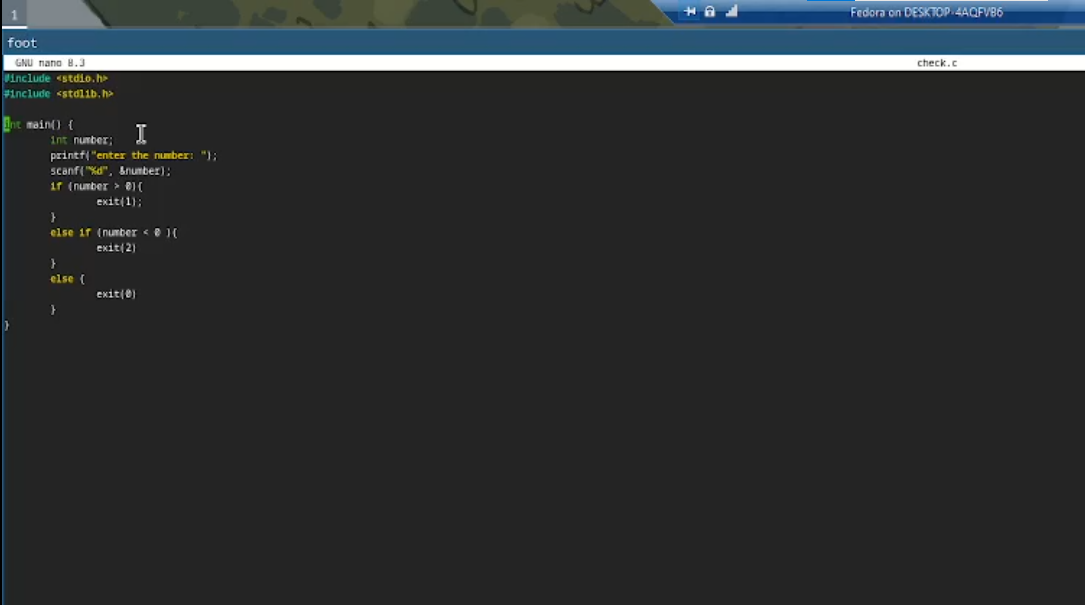
\includegraphics[width=0.7\linewidth,height=\textheight,keepaspectratio]{image/content1.png}

}

\caption{Содержимое тестового скрипта}

\end{figure}%
\end{frame}

\begin{frame}{4.3 Содержимое программы на C}
\phantomsection\label{ux441ux43eux434ux435ux440ux436ux438ux43cux43eux435-ux43fux440ux43eux433ux440ux430ux43cux43cux44b-ux43dux430-c}
\begin{figure}[H]

{\centering 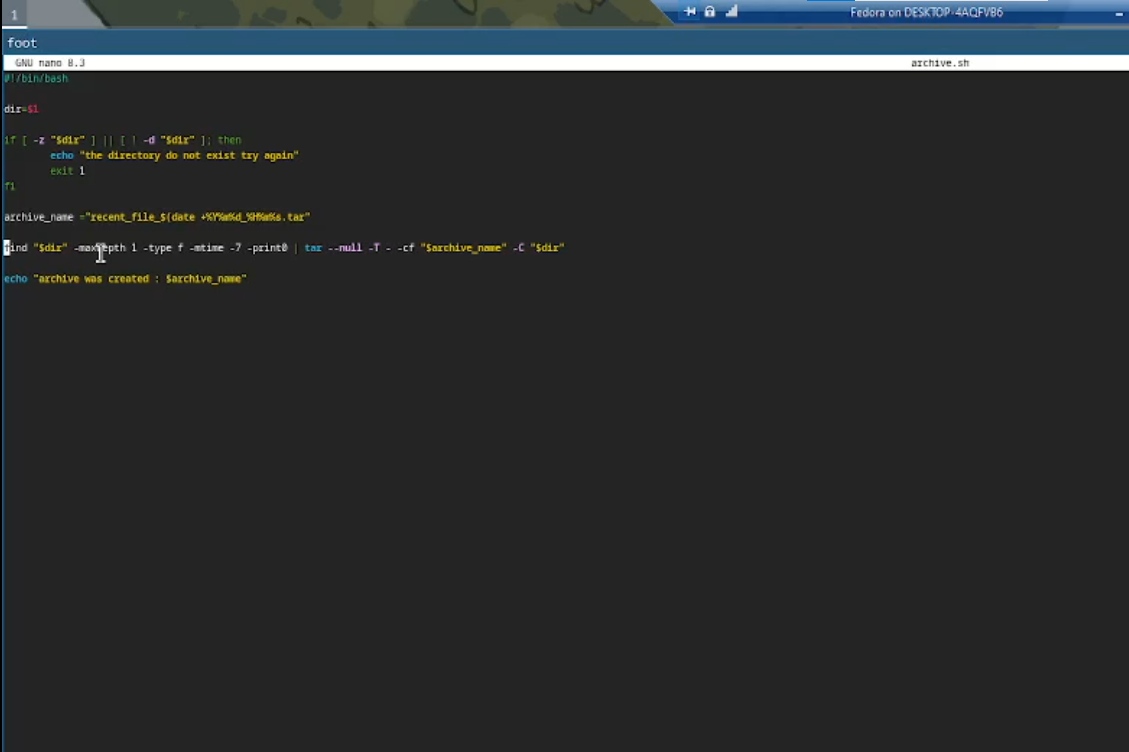
\includegraphics[width=0.7\linewidth,height=\textheight,keepaspectratio]{image/content2.png}

}

\caption{Содержимое программы на C}

\end{figure}%
\end{frame}

\begin{frame}[fragile]{4.4 Компиляция программы}
\phantomsection\label{ux43aux43eux43cux43fux438ux43bux44fux446ux438ux44f-ux43fux440ux43eux433ux440ux430ux43cux43cux44b}
Программа была скомпилирована с различными опциями:

\begin{Shaded}
\begin{Highlighting}[]
\CommentTok{\# Обычная компиляция}
\FunctionTok{gcc}\NormalTok{ test\_program.c }\AttributeTok{{-}o}\NormalTok{ test\_program}

\CommentTok{\# С отладочной информацией}
\FunctionTok{gcc} \AttributeTok{{-}g}\NormalTok{ test\_program.c }\AttributeTok{{-}o}\NormalTok{ test\_program\_debug}

\CommentTok{\# С предупреждениями}
\FunctionTok{gcc} \AttributeTok{{-}Wall} \AttributeTok{{-}g}\NormalTok{ test\_program.c }\AttributeTok{{-}o}\NormalTok{ test\_program}
\end{Highlighting}
\end{Shaded}
\end{frame}

\begin{frame}{4.5 Запуск на переднем плане}
\phantomsection\label{ux437ux430ux43fux443ux441ux43a-ux43dux430-ux43fux435ux440ux435ux434ux43dux435ux43c-ux43fux43bux430ux43dux435}
\begin{figure}[H]

{\centering 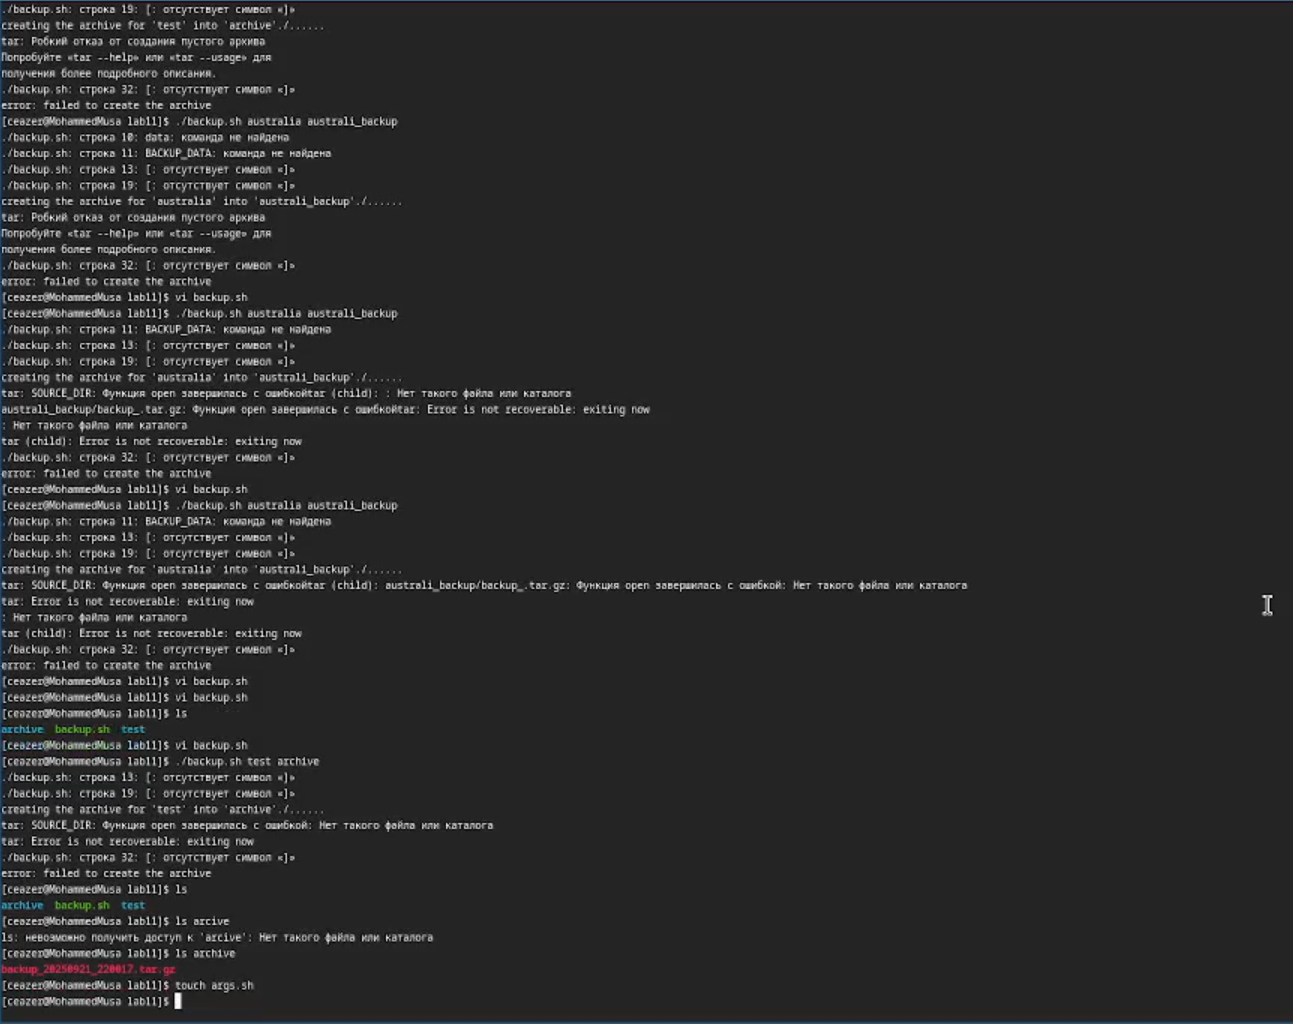
\includegraphics[width=0.7\linewidth,height=\textheight,keepaspectratio]{image/run1.png}

}

\caption{Запуск программ на переднем плане}

\end{figure}%
\end{frame}

\begin{frame}{4.6 Фоновое выполнение}
\phantomsection\label{ux444ux43eux43dux43eux432ux43eux435-ux432ux44bux43fux43eux43bux43dux435ux43dux438ux435}
\begin{figure}[H]

{\centering 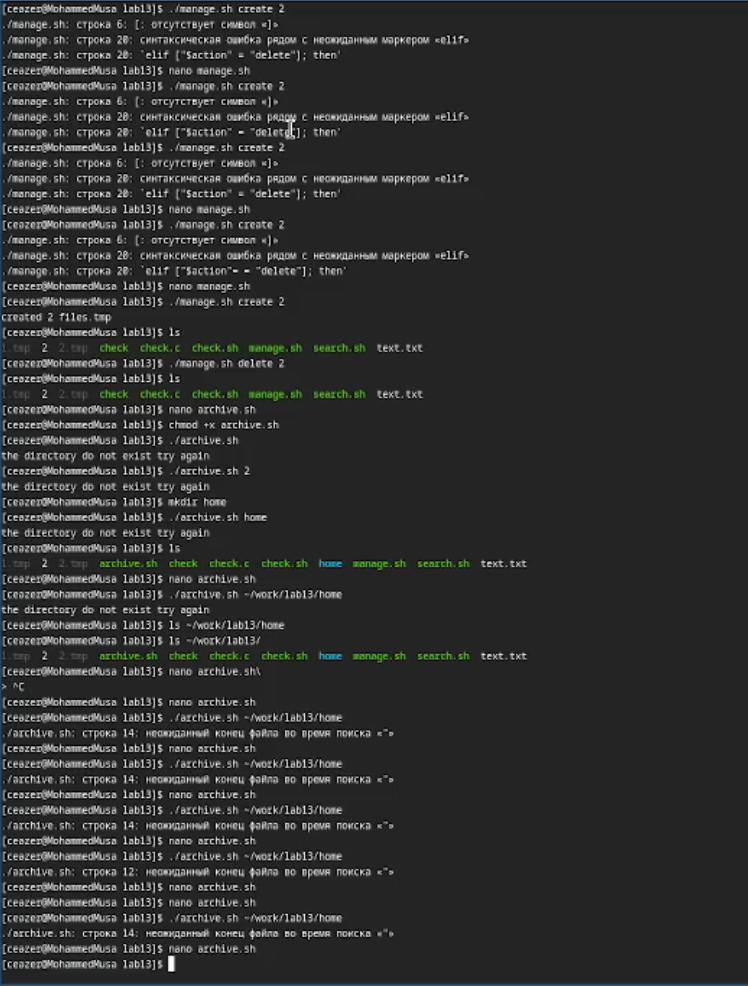
\includegraphics[width=0.7\linewidth,height=\textheight,keepaspectratio]{image/run2.png}

}

\caption{Запуск программ в фоновом режиме}

\end{figure}%
\end{frame}

\begin{frame}[fragile]{4.7 Управление задачами}
\phantomsection\label{ux443ux43fux440ux430ux432ux43bux435ux43dux438ux435-ux437ux430ux434ux430ux447ux430ux43cux438-1}
Практика управления фоновыми задачами:

\begin{itemize}[<+->]
\tightlist
\item
  Запуск программы: \texttt{./test\_program}
\item
  Приостановка: \texttt{Ctrl+Z}
\item
  Продолжение в фоне: \texttt{bg\ \%1}
\item
  Просмотр задач: \texttt{jobs}
\item
  Перевод на передний план: \texttt{fg\ \%1}
\end{itemize}
\end{frame}

\begin{frame}[fragile]{4.8 Перенаправление ввода-вывода}
\phantomsection\label{ux43fux435ux440ux435ux43dux430ux43fux440ux430ux432ux43bux435ux43dux438ux435-ux432ux432ux43eux434ux430-ux432ux44bux432ux43eux434ux430}
Практика перенаправления:

\begin{Shaded}
\begin{Highlighting}[]
\CommentTok{\# Вывод в файл}
\ExtensionTok{./test\_program} \OperatorTok{\textgreater{}}\NormalTok{ output.txt}

\CommentTok{\# Ошибки в файл}
\ExtensionTok{./test\_program} \DecValTok{2}\OperatorTok{\textgreater{}}\NormalTok{ errors.txt}

\CommentTok{\# Оба потока}
\ExtensionTok{./test\_program} \OperatorTok{\textgreater{}}\NormalTok{ output.txt }\DecValTok{2}\OperatorTok{\textgreater{}\&}\DecValTok{1}

\CommentTok{\# Отбросить вывод}
\ExtensionTok{./test\_program} \OperatorTok{\textgreater{}}\NormalTok{ /dev/null }\DecValTok{2}\OperatorTok{\textgreater{}\&}\DecValTok{1}
\end{Highlighting}
\end{Shaded}
\end{frame}

\begin{frame}[fragile]{4.9 Использование конвейеров}
\phantomsection\label{ux438ux441ux43fux43eux43bux44cux437ux43eux432ux430ux43dux438ux435-ux43aux43eux43dux432ux435ux439ux435ux440ux43eux432}
Создание цепочек команд:

\begin{Shaded}
\begin{Highlighting}[]
\CommentTok{\# Поиск процессов}
\FunctionTok{ps}\NormalTok{ aux }\KeywordTok{|} \FunctionTok{grep}\NormalTok{ test\_program}

\CommentTok{\# Подсчет процессов}
\FunctionTok{ps}\NormalTok{ aux }\KeywordTok{|} \FunctionTok{grep}\NormalTok{ test\_program }\KeywordTok{|} \FunctionTok{wc} \AttributeTok{{-}l}

\CommentTok{\# Сортировка по памяти}
\FunctionTok{ps}\NormalTok{ aux }\KeywordTok{|} \FunctionTok{sort} \AttributeTok{{-}k4} \AttributeTok{{-}rn} \KeywordTok{|} \FunctionTok{head} \AttributeTok{{-}10}
\end{Highlighting}
\end{Shaded}
\end{frame}

\begin{frame}[fragile]{4.10 Мониторинг процессов}
\phantomsection\label{ux43cux43eux43dux438ux442ux43eux440ux438ux43dux433-ux43fux440ux43eux446ux435ux441ux441ux43eux432}
Использование инструментов мониторинга:

\begin{itemize}[<+->]
\tightlist
\item
  \texttt{ps\ aux} --- просмотр всех процессов
\item
  \texttt{ps\ -u\ \$USER} --- процессы текущего пользователя
\item
  \texttt{pgrep\ test\_program} --- поиск PID
\item
  \texttt{top} --- интерактивный мониторинг
\item
  \texttt{htop} --- улучшенный мониторинг
\end{itemize}
\end{frame}

\begin{frame}[fragile]{4.11 Отладка bash скрипта}
\phantomsection\label{ux43eux442ux43bux430ux434ux43aux430-bash-ux441ux43aux440ux438ux43fux442ux430}
Отладка с различными опциями:

\begin{Shaded}
\begin{Highlighting}[]
\CommentTok{\# Проверка синтаксиса}
\FunctionTok{bash} \AttributeTok{{-}n}\NormalTok{ test\_script.sh}

\CommentTok{\# Трассировка выполнения}
\FunctionTok{bash} \AttributeTok{{-}x}\NormalTok{ test\_script.sh}

\CommentTok{\# Вывод строк}
\FunctionTok{bash} \AttributeTok{{-}v}\NormalTok{ test\_script.sh}
\end{Highlighting}
\end{Shaded}
\end{frame}

\begin{frame}[fragile]{4.12 Отладка с помощью GDB}
\phantomsection\label{ux43eux442ux43bux430ux434ux43aux430-ux441-ux43fux43eux43cux43eux449ux44cux44e-gdb-1}
Практика отладки программы на C:

\begin{itemize}[<+->]
\tightlist
\item
  Запуск GDB: \texttt{gdb\ ./test\_program\_debug}
\item
  Установка точки останова: \texttt{break\ main}
\item
  Запуск программы: \texttt{run\ arg1\ arg2}
\item
  Пошаговое выполнение: \texttt{next}, \texttt{step}
\item
  Вывод переменных: \texttt{print\ argc}
\item
  Продолжение: \texttt{continue}
\end{itemize}
\end{frame}

\begin{frame}[fragile]{4.13 Трассировка системных вызовов}
\phantomsection\label{ux442ux440ux430ux441ux441ux438ux440ux43eux432ux43aux430-ux441ux438ux441ux442ux435ux43cux43dux44bux445-ux432ux44bux437ux43eux432ux43eux432-1}
Использование strace:

\begin{Shaded}
\begin{Highlighting}[]
\CommentTok{\# Трассировка всех вызовов}
\ExtensionTok{strace}\NormalTok{ ./test\_program}

\CommentTok{\# Вывод в файл}
\ExtensionTok{strace} \AttributeTok{{-}o}\NormalTok{ trace.txt ./test\_program}

\CommentTok{\# Статистика}
\ExtensionTok{strace} \AttributeTok{{-}c}\NormalTok{ ./test\_program}

\CommentTok{\# Только файловые операции}
\ExtensionTok{strace} \AttributeTok{{-}e}\NormalTok{ trace=file ./test\_program}
\end{Highlighting}
\end{Shaded}
\end{frame}

\begin{frame}[fragile]{4.14 Управление приоритетами}
\phantomsection\label{ux443ux43fux440ux430ux432ux43bux435ux43dux438ux435-ux43fux440ux438ux43eux440ux438ux442ux435ux442ux430ux43cux438}
Практика изменения приоритетов:

\begin{Shaded}
\begin{Highlighting}[]
\CommentTok{\# Запуск с низким приоритетом}
\FunctionTok{nice} \AttributeTok{{-}n}\NormalTok{ 10 ./test\_program}

\CommentTok{\# Изменение приоритета}
\VariableTok{PID}\OperatorTok{=}\VariableTok{$(}\ExtensionTok{pgrep}\NormalTok{ test\_program}\VariableTok{)}
\ExtensionTok{renice} \AttributeTok{{-}n}\NormalTok{ 5 }\AttributeTok{{-}p} \VariableTok{$PID}

\CommentTok{\# Проверка приоритета}
\FunctionTok{ps} \AttributeTok{{-}o}\NormalTok{ pid,ni,cmd }\AttributeTok{{-}p} \VariableTok{$PID}
\end{Highlighting}
\end{Shaded}
\end{frame}

\begin{frame}[fragile]{4.15 Завершение процессов}
\phantomsection\label{ux437ux430ux432ux435ux440ux448ux435ux43dux438ux435-ux43fux440ux43eux446ux435ux441ux441ux43eux432}
Различные способы завершения:

\begin{itemize}[<+->]
\tightlist
\item
  \texttt{kill\ \$(pgrep\ test\_program)} --- корректное завершение
\item
  \texttt{kill\ -9\ \$(pgrep\ test\_program)} --- принудительное
\item
  \texttt{killall\ test\_program} --- по имени
\item
  \texttt{pkill\ test\_} --- по шаблону
\end{itemize}
\end{frame}

\section{5. Результаты}\label{ux440ux435ux437ux443ux43bux44cux442ux430ux442ux44b}

\begin{frame}[fragile]{5.1 Выполненные задачи (1)}
\phantomsection\label{ux432ux44bux43fux43eux43bux43dux435ux43dux43dux44bux435-ux437ux430ux434ux430ux447ux438-1}
\begin{itemize}[<+->]
\tightlist
\item
  ✅ \textbf{Освоен запуск программ и скриптов}

  \begin{itemize}[<+->]
  \tightlist
  \item
    Обычный запуск на переднем плане
  \item
    Фоновое выполнение с \texttt{\&}
  \item
    Запуск с \texttt{nohup} для долгих задач
  \item
    Компиляция программ на C
  \end{itemize}
\end{itemize}
\end{frame}

\begin{frame}[fragile]{5.2 Выполненные задачи (2)}
\phantomsection\label{ux432ux44bux43fux43eux43bux43dux435ux43dux43dux44bux435-ux437ux430ux434ux430ux447ux438-2}
\begin{itemize}[<+->]
\tightlist
\item
  ✅ \textbf{Изучено отслеживание выполнения процессов}

  \begin{itemize}[<+->]
  \tightlist
  \item
    Команда \texttt{ps} для просмотра процессов
  \item
    Интерактивный мониторинг с \texttt{top} и \texttt{htop}
  \item
    Поиск процессов с \texttt{pgrep} и \texttt{pidof}
  \item
    Детальная информация о процессах
  \end{itemize}
\end{itemize}
\end{frame}

\begin{frame}[fragile]{5.3 Выполненные задачи (3)}
\phantomsection\label{ux432ux44bux43fux43eux43bux43dux435ux43dux43dux44bux435-ux437ux430ux434ux430ux447ux438-3}
\begin{itemize}[<+->]
\tightlist
\item
  ✅ \textbf{Практикованы инструменты отладки программ}

  \begin{itemize}[<+->]
  \tightlist
  \item
    Отладка bash скриптов с \texttt{-x}, \texttt{-v}, \texttt{-n}
  \item
    Отладчик GDB для программ на C/C++
  \item
    Трассировка системных вызовов с \texttt{strace}
  \item
    Трассировка библиотечных функций с \texttt{ltrace}
  \end{itemize}
\end{itemize}
\end{frame}

\begin{frame}[fragile]{5.4 Выполненные задачи (4)}
\phantomsection\label{ux432ux44bux43fux43eux43bux43dux435ux43dux43dux44bux435-ux437ux430ux434ux430ux447ux438-4}
\begin{itemize}[<+->]
\tightlist
\item
  ✅ \textbf{Освоено управление фоновыми задачами}

  \begin{itemize}[<+->]
  \tightlist
  \item
    Команда \texttt{jobs} для просмотра задач
  \item
    Команды \texttt{fg} и \texttt{bg} для управления
  \item
    Приостановление с \texttt{Ctrl+Z}
  \item
    Завершение с \texttt{kill}, \texttt{killall}, \texttt{pkill}
  \end{itemize}
\end{itemize}
\end{frame}

\begin{frame}[fragile]{5.5 Выполненные задачи (5)}
\phantomsection\label{ux432ux44bux43fux43eux43bux43dux435ux43dux43dux44bux435-ux437ux430ux434ux430ux447ux438-5}
\begin{itemize}[<+->]
\tightlist
\item
  ✅ \textbf{Изучено перенаправление ввода-вывода}

  \begin{itemize}[<+->]
  \tightlist
  \item
    Перенаправление stdout и stderr
  \item
    Конвейеры для связывания команд
  \item
    Использование \texttt{/dev/null}
  \item
    Команда \texttt{tee} для дублирования вывода
  \end{itemize}
\end{itemize}
\end{frame}

\begin{frame}[fragile]{5.6 Дополнительные навыки}
\phantomsection\label{ux434ux43eux43fux43eux43bux43dux438ux442ux435ux43bux44cux43dux44bux435-ux43dux430ux432ux44bux43aux438}
\begin{itemize}[<+->]
\tightlist
\item
  ✅ Управление приоритетами с \texttt{nice} и \texttt{renice}
\item
  ✅ Профилирование с \texttt{time}, \texttt{gprof}, \texttt{valgrind}
\item
  ✅ Точки останова и пошаговое выполнение в GDB
\item
  ✅ Анализ стека вызовов и переменных
\item
  ✅ Создание сложных конвейеров команд
\item
  ✅ Мониторинг использования CPU и памяти
\end{itemize}
\end{frame}

\begin{frame}{5.7 Полученные знания}
\phantomsection\label{ux43fux43eux43bux443ux447ux435ux43dux43dux44bux435-ux437ux43dux430ux43dux438ux44f}
\textbf{Освоены:}

\begin{itemize}[<+->]
\tightlist
\item
  \textbf{Управление процессами} --- запуск, мониторинг, завершение
\item
  \textbf{Фоновое выполнение} --- работа с задачами
\item
  \textbf{Перенаправление потоков} --- управление вводом-выводом
\item
  \textbf{Конвейеры} --- создание цепочек команд
\item
  \textbf{Отладка} --- поиск и исправление ошибок
\item
  \textbf{Мониторинг} --- отслеживание производительности
\end{itemize}
\end{frame}

\section{6. Заключение}\label{ux437ux430ux43aux43bux44eux447ux435ux43dux438ux435}

\begin{frame}{6.1 Выводы}
\phantomsection\label{ux432ux44bux432ux43eux434ux44b}
\begin{itemize}[<+->]
\tightlist
\item
  Освоены методы запуска и управления программами в Linux
\item
  Изучены инструменты отладки и мониторинга процессов
\item
  Получены навыки работы с фоновыми задачами
\item
  Практикованы конвейеры и перенаправление потоков
\item
  Освоены инструменты профилирования и оптимизации
\end{itemize}
\end{frame}

\begin{frame}{6.2 Практическое применение (1)}
\phantomsection\label{ux43fux440ux430ux43aux442ux438ux447ux435ux441ux43aux43eux435-ux43fux440ux438ux43cux435ux43dux435ux43dux438ux435-1}
\begin{itemize}[<+->]
\tightlist
\item
  \textbf{Системное администрирование} --- управление службами и
  процессами
\item
  \textbf{Разработка ПО} --- отладка программ и поиск ошибок
\item
  \textbf{Автоматизация} --- создание скриптов для фоновых задач
\end{itemize}
\end{frame}

\begin{frame}{6.3 Практическое применение (2)}
\phantomsection\label{ux43fux440ux430ux43aux442ux438ux447ux435ux441ux43aux43eux435-ux43fux440ux438ux43cux435ux43dux435ux43dux438ux435-2}
\begin{itemize}[<+->]
\tightlist
\item
  \textbf{Мониторинг систем} --- отслеживание производительности
  приложений
\item
  \textbf{DevOps} --- управление процессами в production окружении
\item
  \textbf{Оптимизация} --- профилирование и улучшение производительности
\end{itemize}
\end{frame}

\begin{frame}{6.4 Значимость навыков}
\phantomsection\label{ux437ux43dux430ux447ux438ux43cux43eux441ux442ux44c-ux43dux430ux432ux44bux43aux43eux432}
Полученные навыки являются \textbf{фундаментальными} для:

\begin{itemize}[<+->]
\tightlist
\item
  Эффективной работы в Linux
\item
  Системного администрирования
\item
  Разработки программного обеспечения
\item
  DevOps и автоматизации
\end{itemize}
\end{frame}

\begin{frame}[standout]{6.5 }
\phantomsection\label{section}
Спасибо за внимание!
\end{frame}




\end{document}
